\chapter*{Introduction}
\addcontentsline{toc}{chapter}{Introduction}
This dissertation focuses on the work conducted on the SIRIUS storage ring with the objective of optimizing the ring's \gls*{DA} and \gls*{ie}. The text is structured as follows:
\begin{itemize}
    \item The current chapter introduces synchrotron light sources, provides an overview of the SIRIUS project, outlines the main components and subsystems present in electron storage rings, and elucidates the problem addressed in this work;
    \item Chapter 1 delves into the theoretical and scientific background regarding the dynamics of particles in accelerators. It covers topics such as optics functions, tunes, chromatic effects, field errors, perturbations, and the dynamic aperture;
    \item Chapter 2 introduces the online optimization of nonlinear dynamics in accelerators and presents the \gls*{RCDS} algorithm;
    \item Chapter 3 presents the diagnostic tools available for probing the electron beam's motion, current, and other relevant parameters. It also covers technical details on the design of the experiments and measurements reported here, such as the choice of the objective function and the decision variables for the optimization problem;
    \item Chapter 4 presents the results of the online optimization experiments and discusses their significance for the machine operation and stability.
    \item Lastly, Chapter 5 provides conclusions and closing remarks on the findings and implications of the study.
\end{itemize}

\section*{Storage ring-based synchrotron light sources}
\addcontentsline{toc}{section}{Storage ring-based synchrotron light sources}

\gls*{sr} is the electromagnetic radiation emitted by charged relativistic particles when accelerated perpendicularly to their motion. The phenomenon was theoretically predicted in the early 1900s when Liénard and Wiechert calculated the retarded potentials for point particles. The first experimental observation occurred at General Electric's synchrotron accelerator, justifying the adoption of the term "synchrotron" in its name \cite{wiedemann_particle_2015}.

Synchrotron light is extremely collimated and has a broad spectral distribution, covering from infrared to hard X-rays. These properties make it ideal for imaging experiments in crystallography and spectroscopy across a wide variety of scientific disciplines.

Modern synchrotron light sources rely primarily on two particle acceleration technologies: free-electron lasers and electron storage rings. Here we focus on storage ring-based synchrotron light source facilities. In these facilities, ultra-relativistic electron beams are stored for extended periods in a closed orbit within a chamber in ultra-high vacuum to produce synchrotron light. The beam is maintained in stable orbits by the fields of magnets carefully placed along the ring to provide bending and focusing of the electrons trajectories. It is also periodically influenced by longitudinal standing-wave electric fields in the radio-frequency range, which replenish the energy radiated away in the form of light.

The main figure of merit for measuring the quality of a \gls*{sr} source is the \textit{brightness}\cite{huang_brightness_2013}, defined as the photon flux density in phase space \cite{hettel_challenges_2014,wiedemann_particle_2015}:
\begin{equation}
    B(\omega) = \frac{1}{\Delta \omega/\omega}\frac{\dot{N}(\omega)}{4\pi^2\Sigma_{x}(\omega)\Sigma_{y}(\omega)},
\end{equation}
where $\dot{N}$ is the photon flux at energy $E=\hbar\omega$, $\Sigma_{u}$ is the photon beam volume in the $u=x,y$ phase space, and $\Delta\omega/\omega$ is the frequency bandwidth. The photon phase space volume depends on the convolution of the electron beam distribution with the distribution of the photons emitted by a single electron. The latter depends on the photon energy and the emission process, while the former is related to the phase space volume of the electron beam: the \textit{emittance}. The equilibrium beam emittance depends on the magnetic lattice and has units of the transverse phase space areas (size $\times$ angle). Increasing brightness can be achieved by maximizing the photon flux, reducing the electron beam emittances and optimizing the matching between photon and electron beams distribution orientation. \cite{wiedemann_particle_2015}.
%From the perspective accelerator scientists and engineers, in general, the most used figure of merit for synchrotron machines is the emittance rather than brightness.

Synchrotron light sources can be classified based on their brightness and emittance. In the early 1960s, the community interested in \gls*{sr} for imaging experiments obtained it parasitically from high-energy and nuclear physics machines such as \acrshort*{desy} and \acrshort*{doris}, in Germany, and ADA, in Italy \cite{simoulin_synchrotron_2016}, marking the era of first-generation synchrotron light sources \cite{liu_towards_2017}. The second-generation machines emerged in the 1980s and consisted on machines designed exclusively for \gls*{sr} production, such as \acrshort*{bessy}, \acrshort*{doris} II, \acrshort*{doris} III, and \acrshort*{elsa}, in Germany; \gls*{SuperACO}, in France; MAX I, in Sweden \cite{simoulin_synchrotron_2016}; \acrshort*{nsls} and \acrshort*{spear}, in the USA; \gls*{UVX} in Brazil; \gls*{kek} Photon Factory and \gls*{SOR-Ring}, in Japan.

The 1990s saw a growing demand for higher brightness, leading to the development of third-generation machines \cite{liu_towards_2017}. These machines introduced \glspl*{id} such as wigglers and undulators, which consist of a sequence of alternating magnetic fields generally created by an array of permanent magnets arranged in a Halbach array. \glsplural*{id} significantly enhance brightness by adding the radiation emitted by many poles. They also allowed precise control over the emitted radiation energy and polarization.

Typical emittances for third-generation machines is of the order of units to tens of $\unit{nm}.\unit{rad}$. Most of the currently operating machines pertain to the third-generation, such as \gls*{alba}, in Spain; \acrshort*{soleil} and \acrshort*{ESRF}, in France; Diamond, in the United Kindom; \gls*{ELETTRA}, in Italy \cite{simoulin_synchrotron_2016}; \acrshort*{spear}3, \acrshort*{APS}, \acrshort*{ALS} and \acrshort*{nsls}-II, in the USA.

The era of the \glspl*{4gsr} commenced with the design of the MAX-IV machine in Lund, Sweden, in 2015 \cite{liu_towards_2017,hettel_challenges_2014}. \glsplural*{4gsr} achieved a notable reduction in emittance, reaching sub-$\unit{nm}.\unit{rad}$ values thanks to recent technological advancements in accelerator technology, such as computer simulations, vacuum technology, machining, mechanical alignment, and others  \cite{hettel_challenges_2014,liu_towards_2017}. Following MAX-IV, an upgrade of the \acrshort*{ESRF} facility, the ESRF-EBS, in France, and the launch of SIRIUS, in Campinas, Brazil, marked significant milestones for the fourth-generation. Today, several \gls*{4gsr} projects are being planned, designed and constructed around the globe.

\section*{The SIRIUS project}
\addcontentsline{toc}{section}{The SIRIUS project}

SIRIUS is a \gls*{4gsr} synchrotron light source. It was designed, built, and is operated by the \gls*{lnls}, on the campus of the \gls*{cnpem}, in Campinas, Brazil. The electron storage ring has $518~\unit{m}$ in circumference and its operating energy is $3~\unit{GeV}$. The natural emittance of the lattice is $250~\unit{pm}.\unit{rad}$.
% It is expected to reach up to $150~\unit{pm}~\unit{rad}$ with the installation of the machine's definitive IDs \cite{liu_synchrotron_2019}\footnote{SIRIUS is currently operating with provisional IDs for providing light to the first users and allowing scientific commissioning of the beamlines}.

SIRIUS succeeded the first synchrotron light source in Brazil, the UVX machine, which opened to users in 1997 and served the community until its shutdown, in the beginning of SIRIUS commissioning, in August 2019
%\footnote{The UVX project led to the creation of \gls*{lnls}, which marked a new model for scientific research in Brazil, based on social organizations under contracts with the Ministry of Science Technology and Innovations. LNLS paved the way for national labs, including labs on bio-sciences (LNBio), nanotechnology (LNNano), and bio-renewables (LNBR), which are also located at the CNPEM campus.}
\cite{liu_synchrotron_2019}. The SIRIUS project started in 2009, initially planned and designed as a third-generation machine. By 2012, the project evolved into that of a \gls*{4gsr} \cite{liu_synchrotron_2019}. Building construction was finished in 2018, the \acrshort*{linac} and Booster commissioning soon followed. In November 2019 the first beam was stored in the storage ring.

SIRIUS finished the Phase-0 commissioning in 2022 and since March 2023 is receiving the first external users. At the time of this writing, \todo{check this info} it has 10 operating beamlines, 1 beamline in commissioning, 2 under construction and 1 beamline in design\cite{lnls_beamlines}. The storage ring currently stores $100~\unit{mA}$ current, operating with frequent beam injections throughout the day, a scheme known as ``top-up'' mode. SIRIUS is expected to achieve $350~\unit{mA}$ current when the system of two superconducting \gls*{rf} cavities and the third-harmonic cavity are installed \cite{liu_status_2022,liu_status_2023}.

Presently, SIRIUS stands as the most complex scientific infrastructure ever constructed in Brazil, aiming to position the country at the forefront of global leadership in synchrotron light science and technology. It has the capacity to host up to 40 beamlines and as of the time of this writing, SIRIUS is the sole fourth-generation synchrotron light source in the southern hemisphere and one of merely three \glsplural*{4gsr} in operation across the globe.

\section*{Physics of electron storage rings: an overview}
\addcontentsline{toc}{section}{Physics of electron storage rings: an overview}

Typical systems comprising a storage ring synchrotron light source facility include:
\begin{itemize}
    \item an injection system: including the electrons source, beam transport lines, the linear accelerator and the booster synchrotron accelerator. At SIRIUS, the linear accelerator provides the booster with a $150~\unit{MeV}$ beam. The booster further ramps the beam energy up to $3~\unit{GeV}$, which is the storage ring operation energy;
    \item storage ring: where the ultra-relativistic beam of electrons is kept in stable orbits for hours within the vacuum-chamber, producing synchrotron light at the bending magnets and insertion devices;
    \item beamlines which steer the photon beams towards the experimental cabins where samples are placed for the experiments based on light-matter interaction, such as spectroscopy, crystallography, tomography and others.
\end{itemize}
A schematic view of the SIRIUS building is shown in Fig.~\ref{fig:sirius_layout}.
\begin{figure}[tb]
    \centering
    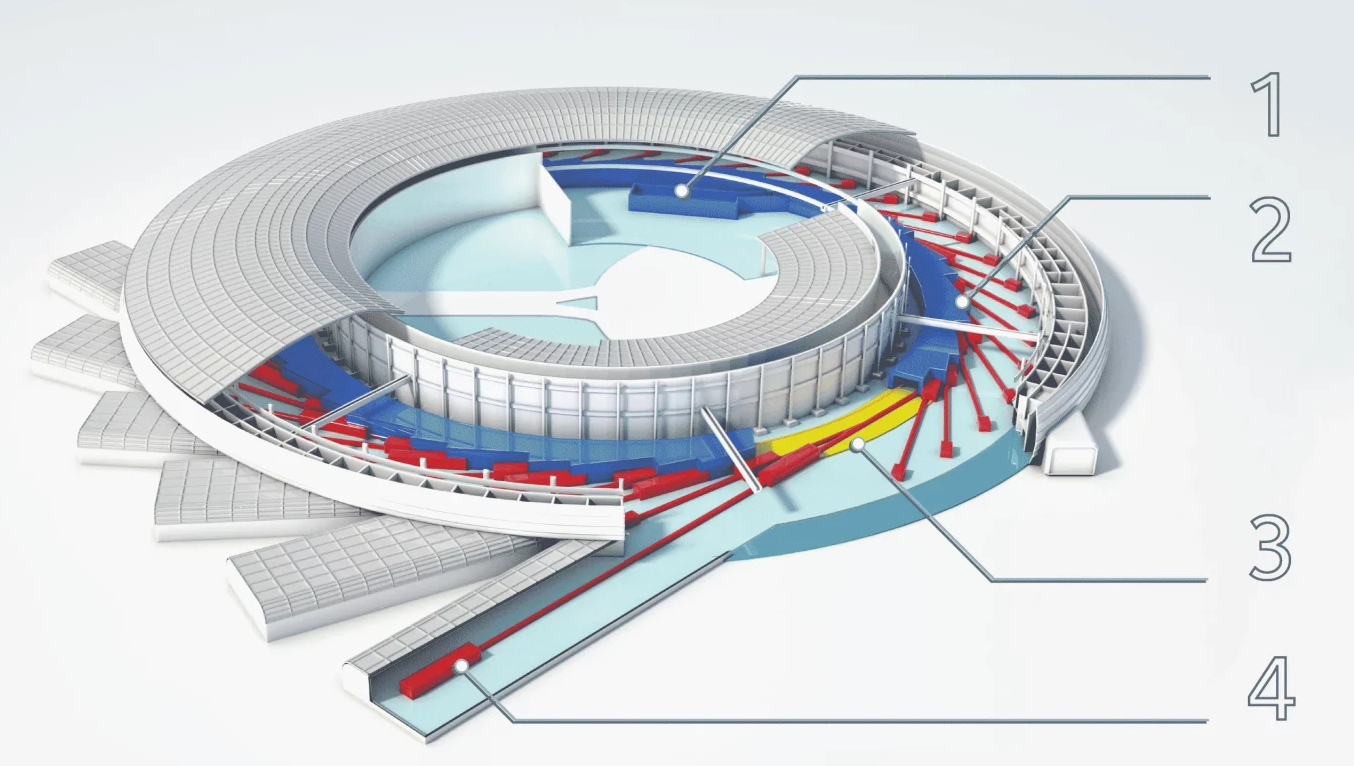
\includegraphics[width=0.8\textwidth]{Images/sirius_facility.png}
    \caption[Schematic view of the SIRIUS installations.]{Schematic view of the SIRIUS installations. 1) \gls*{linac}; 2) Concrete tunnel housing the booster accelerator and the storage ring; 3) storage ring; 4) beamlines. From \href{https://lnls.cnpem.br/sirius/como-funciona-o-sirius/}{\gls*{lnls} website}.}
    \label{fig:sirius_layout}
\end{figure}

\begin{figure}[tb]
    \centering
    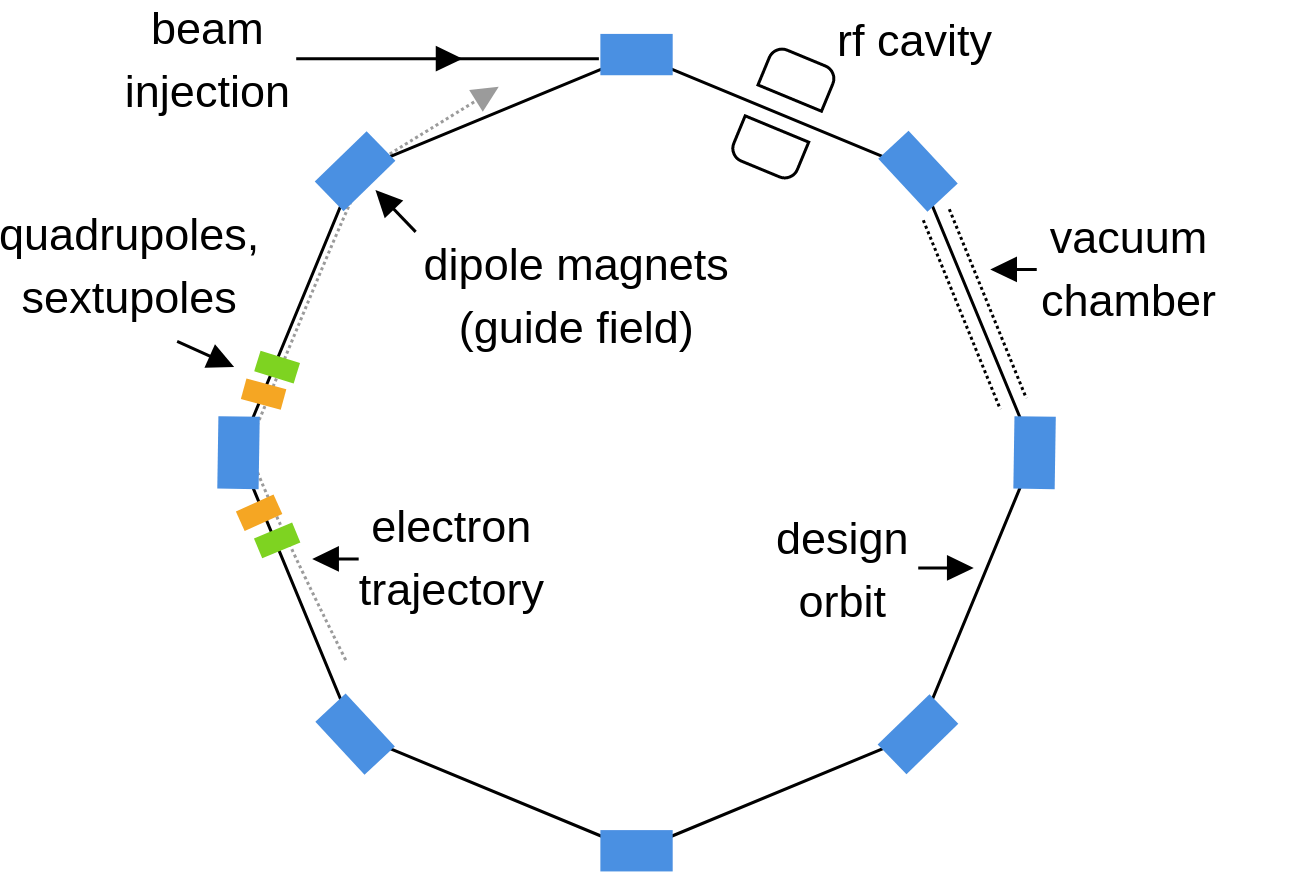
\includegraphics[width=0.6\textwidth]{Images/storage_ring.png}
    \caption[Storage ring typical configuration.]{Storage ring typical configuration. Inspired by ref.~\cite{sands_physics_1969}}
    \label{fig:storage_ring}
\end{figure}
Figure~\ref{fig:storage_ring} outlines the typical layout of a synchrotron storage ring. The electron beam is stored within a vacuum chamber, where the individual electrons oscillate in proximity to a reference closed orbit, under the influence of magnetostatic fields from an array of multipolar magnets --the lattice, and also time-dependent fields from the \gls*{rf} cavities. The orbit circumference is determined by the strengths of the deflection magnets, the dipoles, and the operational energy of the beam.

A pure dipole magnet provides a uniform and homogeneous magnetic field perpendicular to the facility floor and bends the electron's trajectory in the plane parallel to the floor. The field profile of a dipole magnet is depicted in the left-side sketch of Fig.~\ref{fig:magnets_fields}. Imagining a beam directed inward toward the screen, the trajectory will be bent to the right. For trajectories resulting in a closed orbit, the overall bending angle provided by the dipoles along the entire ring must equal $2\pi$ radians.

To maintain electrons in close proximity to the reference orbit, focusing of the trajectories is required. Focusing is attained by employing gradient fields, primarily generated by quadrupole magnets at SIRIUS. The strength of such fields increase linearly with deviations from the closed orbit, which lies in the magnet's center. Gradient fields effectively act as restoring spring forces. The magnets poles and the field profile of a quadrupole magnet are depicted in the center sketch of Fig.~\ref{fig:magnets_fields}.

Focusing and deflection are energy-dependent, which means small deviations from the nominal operating energy can result in a enlarged or reduced orbit and on differential focusing at the gradients. The former effect is a dispersion effect, while in the latter, drawing an analogy from geometric optics, the beam's focusing behavior at the "lens" (quadrupoles) depends on its "color" (energy). To correct for these chromatic aberrations the sextupole fields serve as corrective lenses. They introduce geometric aberrations to counteract the chromatic ones, resulting in approximately uniform, energy-independent focusing, up to the linear approximation. The magnets poles and the field profile of a sextupole magnet are depicted in the right sketch of Fig.~\ref{fig:magnets_fields}.

Besides dipoles, quadrupoles and sextupoles, additional dipole actuators magnets for orbit/trajectory correction and pulsed magnets for beam injection can also be found in the ring.
\begin{figure}[htb]
    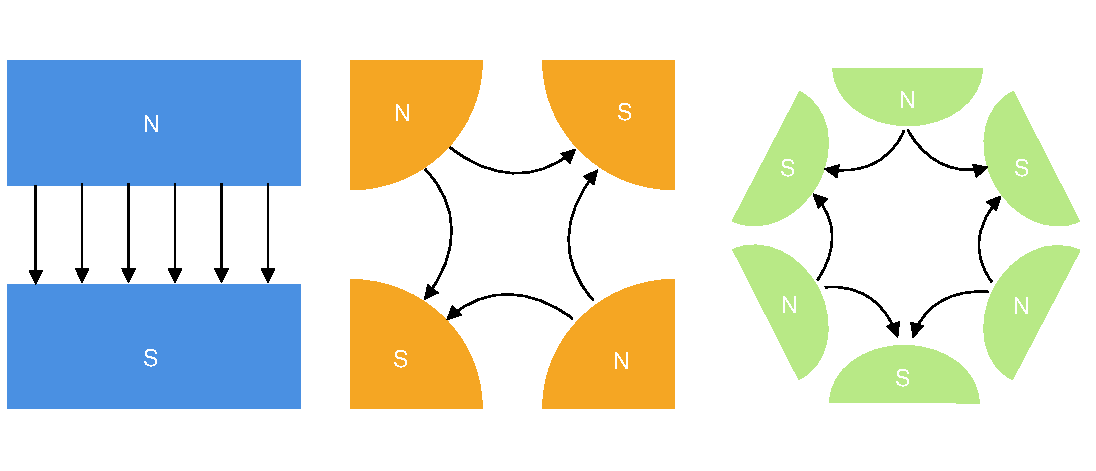
\includegraphics[width=\textwidth]{Images/magnets.pdf}
    \caption[Schematic representation of the magnets comprising SIRIUS lattice and their fields profile.]{Schematic representation of the magnets comprising SIRIUS lattice and their fields profile. From left to right: dipole magnet, quadrupole magnet and sextupole magnet.}
    \label{fig:magnets_fields}
\end{figure}
%As mentioned previously, a storage ring is designed to confine bunches of electrons and steer them along a reference closed orbit. The orbit is defined by the bending magnets, the dipoles. The trajectories consist on oscillations about the closed orbit, and focusing of such oscillations toward the closed orbit is provided by gradient fields, mostly coming from quadrupole magnets. Additionally, to correct chromatic aberrations in the beam's motion, i.e. a dependence of focusing with the beam's energy, and guarantee correct focusing despite energy deviations from the nominal value, sextupolar magnetic fields are also introduced, providing fields depending qudratically on the deviations from the nominal orbit. These fields introduce strong nonlinearities in the dynamics.

When having its trajectory bent at the dipoles and insertion devices,
%\footnote{Insertion devices (IDs) consist on arrays of magnetic blocks arranged to provide additional deflection of the beam's trajectory for the production of synchrotron radiation. IDs allow for fine-tuning of the fields and as consequence of the characteristics of the emitted readiation, such as the energy and polarization.}
the beam loses energy in the form of synchrotron radiation. To avoid inward spiraling and maintain the beam stored, the energy lost must be replenished. To achieve this, \gls*{rf} cavities are placed along the ring to provide oscillating electric fields along the longitudinal direction. The work done in the beam by the fields restore its energy.

The radiated photons are emitted in a narrow cone with angular aperture of $1/\gamma$, $\gamma$ being the relativistic Lorentz factor ($\sim 6000$ at SIRIUS storage ring). The photons carry away a fraction of the beam's momentum in both the longitudinal and transverse directions. However, when passing through \gls*{rf} cavities, only momentum in the longitudinal direction is replenished. The combined effect of radiating photons and passing through \gls*{rf} cavities leads to an overall damping of the transverse oscillations amplitudes.

On the other hand, the quantum nature of the emitted radiation leads to the excitation of transverse oscillations, an effect known as quantum excitation. When a photon carries away energy, it depletes the electrons energy by the same amount. It thus changes the reference orbit of the electron because of the dispersion effect, inducing oscillations. Additionally, coupling on the transverse plane and intra-beam scattering events can lead to the excitation of transverse oscillations, enlarging the beam size.
%Additionally, the very fact that radiation is emitted within a finite angular aperture means that, by momentum conservation, the emission of a photon is accompanied by a transverse recoil. These two mechanisms are responsible for the excitation of transverse oscillations.
Eventually, equilibrium between radiative damping and transverse excitations is achieved, leading the beam size to reach a stationary value

Each degree of freedom of the beam defines an acceptance, which establishes limits on the dynamical variables. Exceeding these limits can result in unstable, unbounded motion, and eventually, beam losses. The most apparent form of acceptance is the transverse acceptance, since the beam motion is bounded by a vacuum chamber, and colliding with the chamber's physical aperture leads to losses. Additionally, the beam has an energy acceptance, representing a tolerance for energy deviations from the nominal value. Exceeding this tolerance can lead to a sub-optimal energetic balance when passing at the \gls*{rf} cavities. On the span of several turns, the energy deviations can grow and result in significant deviations from the nominal orbit because of the dispersive effect. Eventually the beam collides with the vacuum chamber wall.

Because of the nonlinearities introduced by the sextupole magnets, the transverse acceptances can be limited not solely by the physical aperture available in the vacuum chamber but rather by the amplitudes above which motion is irregular, unstable and unbounded. This limiting amplitude is known as the \gls*{DA}, a term that can be used to refer to the limiting amplitudes in the transverse space $x,y$ as well as the phase space coordinates $x, p_x$ and $y, p_y$.

The acceptances and the expected rate at which anomalies in the degrees of freedom can occur define a base rate for the expected beam loss in the ring. The beam is also susceptible to elastic and inelastic collisions with residual gas molecules within the chamber, as well as collisions between electrons within the same bunch. All these effects can lead to beam losses, and the overall beam loss rate resulting from these combined mechanisms defines the characteristic time scale at which a given electron current survives in the ring. This is the beam lifetime and determines the rate at which injections into the storage ring are required to maintain the current within a specified range.

\section*{The problem addressed in this work}
\addcontentsline{toc}{section}{The problem addressed in this work}

The pursuit of low emittances and high brightness has propelled the accelerator community toward the fourth-generation of storage rings. Achieving such low emittances was made possible by a series of technological advances that enabled the use of the \gls*{mba} lattice\cite{liu_towards_2017,hettel_challenges_2014}. \gls*{mba} lattices require intense gradient fields provided by quadrupole magnets, which, in turn, demand the presence of strong sextupolar fields to compensate for chromatic effects. As sextupoles introduce nonlinear fields, the dynamics in fourth-generation storage rings has become increasingly nonlinear\cite{liu_towards_2017}.

A quasi-periodic nonlinear dynamics when subjected to perturbations, such as small field errors stemming from rotation, alignment, or fields excitation errors, can potentially become unstable at large oscillation amplitudes. These instabilities impose constraints on the maximum transverse oscillation amplitudes that the machine can accommodate, the \gls*{DA} of the ring. Exceeding the \gls*{DA} results in irregular and often chaotic motion and beam loss.

Under normal operation conditions, the equilibrium beam size and the typical oscillation amplitudes are considerably smaller than the \gls*{DA} , and the dynamics can be well studied and analyzed using a linear approximation theory, without worrying about the \gls*{DA}. However, there are specific scenarios where the \gls*{DA} becomes crucial for the operation, notably during the injection process.

During injection into the storage ring for beam accumulation, the beam is extracted from the booster accelerator and guided toward the storage ring through a transport line. Upon entering the ring, the beam is deflected by the field of a pulsed nonlinear magnet, aligning the beam almost parallel to the storage ring tangent direction, albeit with a horizontal offset of approximately $x=-8~\unit{mm}$ \cite{liu_injection_2016}. If the \gls*{DA}  is smaller than this initial amplitude, it imposes limitations on the \gls*{ie}.

The \gls*{DA} is determined by the beam's nonlinear dynamics performance, which is a consequence of the nonlinear lattice (sextupoles). In the design phase of the SIRIUS project, the placement, symmetry, and strength of sextupole magnets were determined through a multi-objective optimization process, primarily focused on improving the simulated \gls*{DA} and beam lifetime of the machine's computer model\cite{de_sa_optimization_2016, dester_energy_2017}. This optimization work considered the average performance of the lattice configurations while accounting for various magnet errors that simulate the expected errors in the actual machine \cite{de_sa_optimization_2016}. Several models, with errors distributed among the magnets, were generated, and the \gls*{DA} and lifetime for a given lattice configuration were calculated by simulating the electron beam's motion for thousands of turns (tracking simulations). The final figure of merit for a magnetic lattice consisted of the average \gls*{DA} and lifetime it provided to the ensemble of machines. The best-performing machine lattice found during this process was adopted as the nominal lattice and subsequently deployed during the commissioning phase of the machine. Prior to the optimization work reported here, the machine operated with this nominal sextupole configuration.

The real machine consists of a practical realization of a specific error configuration, which defines the physically realized magnetic lattice and determines the overall performance of the dynamics. The nominal nonlinear lattice, identified as the best-performing lattice on average in simulations, is not necessarily the optimum lattice for this specific error realization.

Assuming the realized lattice closely approximates the optimum setup, i.e., that the errors are small, it is reasonable to assume that by making minor tweaks and adjustments to the sextupoles, one can adapt the nonlinear lattice the actual distribution of errors in the physical system. Since the sextupoles are already installed, the optimization variables available are their field strengths. A fine-tuning of strengths aiming to accommodate the nonlinear fields to the realized lattice can result in improvements to the nonlinear dynamics performance, increases in the \gls*{DA}, and an enhancement of \gls*{ie}.

This process has already been demonstrated in other machines \cite{huang_algorithm_2013, huang_online_2015,liuzzo_rcds_2016,olsson_online_2018, yang_online_2022}. It has proven to be a successful approach and became known as \textit{Online optimization}. If one thinks of the errors as agents that deteriorate the DA from its optimum, online optimization can be seen as an attempt to compensate for such deterioration. Online optimization of the machine nonlinear dynamics consists of employing computer-automated search strategies to systematically explore various sextupole configurations with the goal of identifying the ones that yield the largest DA while not interfering with other machine parameters, such as chromaticity and beam lifetime. The key ingredient in online optimization is the choice of a robust optimization algorithm based on direct or indirect search in the parameter space. The most widely used is the \gls*{RCDS} algorithm \cite{huang_algorithm_2013}, which is based on a noise-robust one-dimensional optimizer along with a clever strategy, known as Powell's method, for choosing directions in the search space. Chapter 2 addresses the RCDS algorithm.

Besides improving the \gls*{DA} and \gls*{ie} in nominal operation conditions, it is also interesting, and in some cases it is necessary, to do so in different machine \textit{working points}, with different \textit{tunes}. As presented in chapter 1, if one fixes one's attention to a specific point of the ring, and measure the beam position in horizontal and vertical planes for consecutive turns, one realizes the motion is a sampled sinusoid and the fractional parts of the tunes $\nu_x$ and $\nu_y$ are the fundamental frequencies of such harmonic motion on each plane. The tunes are important operation parameters and influence the response of the beam in the presence of perturbations. Tunes close to integer numbers result in large \textit{orbit amplification factors} making the dynamics particularly sensitive to perturbations. The fractional parts of SIRIUS nominal tunes are quite low, and increasing them would distance the tunes away from integer numbers, reducing the orbit amplification factors and improving orbit stability.

Changing the tunes can be achieved by actuating with the quadrupole magnets, but doing so takes the machine to a different operating optics, in which the DA can, and often is, smaller than the \gls*{DA} in nominal tunes. In different working points, thus, online optimization is essential to find a new sextupole configuration to adapt the nonlinear magnets to the new optics and achieve a good DA and acceptable \glspl*{ie} for operation.

In agreement with the experience in other facilities, it is shown in Chapter 4 that online optimization using \gls*{RCDS} can successfully improve the dynamics performance and lead to \gls*{DA} and \gls*{ie} improvements. This was observed for the SIRIUS storage ring both in the machine nominal tunes as well as in other working points, with tunes with higher fractional parts.  SIRIUS experience with online optimization is a valuable demonstration of this tool's efficiency in fourth-generation rings, specially because SIRIUS has so many sextupole magnets and thus such a large search space.

At the time of this writing, SIRIUS is operating with the sextupole configurations found during the experiments carried out while executing this project \cite{velloso_online_2023}. The configuration was found by online optimizing the machine with increased tunes. The higher tunes led to a reduction in orbit amplification factors, resulting in unprecedented orbit stability \cite{liu_status_2023}.

In the upcoming chapter, the dynamics of electrons in storage rings is examined. The linear approximation theory is introduced, and nonlinear dynamics is treated as a perturbation to the linear theory. The goal is to introduce the optics functions and relevant quantities such as chromaticity and dispersion, and to present how a nonlinear dynamics is limited by the increase in instabilities and irregularities at large amplitudes. Chapter 2 provides a brief overview of optimization strategies and focuses on familiarizing the reader with the \gls*{RCDS} algorithm. Chapter 3 presents the methods, measurement procedures and diagnostics tools available and required for the execution of the online optimization experiments and Chapter 4 presents the results of the optimization at the SIRIUS storage ring.
